\documentclass[11pt]{article}
\usepackage{fullpage}
\usepackage{graphicx}

\title{CS63 Spring 2019\\Earthquake Prediction}
\author{Theo Schrader, Ethan Zhao, Kieran Huang}
\date{5/2/19}

\begin{document}

\maketitle

\section{Introduction}

In this project, we are tackling a Kaggle challenge called "LANL Earthquake Prediction." In the problem,
we are given a dataset full of seismic data (approximately, the acoustic variance of seismic waves) as well as time to next fault failure (earthquake) and are tasked to predict,
given seismic data, the approximate imminence of an earthquake. In order to tackle this problem,
we use Keras to construct a long short term memory (LSTM) recurrent neural network (RNN) to
predict the earthquake imminence. Preceding LSTM layer, we included a 1D ConvNet layer to detect features
within the data.

We decided to use an LSTM because the network deals well with time-series style data, in which
each previous input influences the next one. This works well with our data, as the time-to-failure(TTF), the time until the next earthquake, cannot be realistically predicted by any particular data point but only by looking an ordered temporal sequence of many. Additionally,
the LSTM gives us the potential to predict upcoming acoustic data, which can be used to refine the model's predictions further based
on their accuracy (i.e. erroneous TTF predictions can be used to refine the model as well as incoming seismic data predictions that 
don't match the data received).

In our problem, we decided to discretize our output, predicted time-to-failure, into three categories of how close
it was to an earthquake: highly critical, fairly critical, and not critical. This way, we have a clearer and more straightforward
system that neatly sorts our output into simple and understandable categories, allowing the results to be interpreted more easily
by a human. 

\section{Method and Details}


Our data was made up of lines of seismic signal data (voltage), each corresponding to a TTF. In order to properly assess the causal nature of the time series data, we arranged the input (the seismic data)into sequences of temporally-ordered
values. For our final model, each of these sequences constituted one input into the ConvNet, which then outputted further data that was passed into the LSTM to train the network to recognize the
discretized category each sequence corresponded to. In between, we also had two dense layers, one to analyze the results of the LSTM further and the other
as an output layer with three output nodes (one for each category of output).

We first took careful looks at our given dataset in order to make decisions of how to prepare and organize our data. We printed out several graphs depicting
the data and looked at a helpful kernel on the Kaggle page further explaining details about the data (Shaking Earth by Allunia) and found that
within the billions of data points, there were actually only 16 earthquakes that occurred. Thus, we decided to shrink the data we used to only a fraction of this data (approximately 1/4)
and also make other decisions when organizing the data, namely putting them into sequences into length 100. Further, instead of overlapping sequences
so that each subsequent 100-long sequence started just one after the start of the previous one, as suggested by the example given by Professor Meeden, we decided to make the first value of each subsequent sequence directly follow the last value of the previous sequence. This way, we could analyze more of the data set and do
it in a more efficient and timely manner to allow for more frequent testing. If we allowed the data to overlap so that each subsequent sequence overlapped almost entirely with the previous, we would have had a completely overwhelming amount of data to process and work with, while not actually being able to look at the entire dataset more comprehensively and holistically.

In order to discretize our output, we initially converted each time-to-failure value into one of the three category markers. The cutoffs were as such:
0-3 seconds to failure was highly critical, 3-6 seconds was medium critical, and 6+ seconds was not critical. To decide on these categories, we
made careful analyses of the raw data, using Matlab in python to print graphs depicting the shape of our data. In these graphs, we saw that
these numbers gave an approximately even distribution (about a third of the data fell into each category). Because 
evenly distributed outputs would more fairly test the model's ability to predict imminence and allow us to understand its accuracy as a variance from 33\% (random guessing), we thought classifying the output in this manner would be the best course of action.

In order to make sure our LSTM was learning properly, we randomized our sequences and output categories (making sure that when shuffled, these two corresponding values would still align in each index) so that the neural network would not overfit and merely aim to predict the linearly decreasing nature of time to failure in the dataset. By randomizing the arrays, we were able to let the LSTM actually more actually predict earthquake imminence critical values that weren't just aligned to the time before one earthquake.

Finally, we separated our dataset into training and test sets in a 90-10\% ratio so that we could train our dataset appropriately with a large and diverse enough set of values, but also be able to test a diverse set of examples as well to get an accurate gauge of how well our LSTM did.

For our LSTM, we tested multiple activation, loss, and optimizer functions, starting first with softmax, categorical crossentropy, and SGD (commonly used functions that we had used prior for the MNIST dataset) before landing on "selu" as our activation function and "Nadam" as our optimizer. We had tested extensively many
different activation functions and optimizers for each and found that these gave us the best results.

After running the LSTM and getting an initial accuracy value (starting at around 53\%), we tried several different methods of improving the results of our LSTM.

The first improvement we tried making to the LSTM was to manually add in features as additional one-hot inputs into the LSTM, so that hopefully, the network could learn from these features and learn to weigh these features accordingly in making its decisions. These features we added were mathematical calculations on our sequences that could provide succinct and summarizing information about our sequences, and following this logic, we ended up adding 7 features: the Sum, Min, Max, 25th percentile, 50th percentile, 75th percentile and Average. We calculated these features for each sequence and appended them to a list of features.

A second improvement we tried was creating a ConvNet to create features for the LSTM. The ConvNet was built into the LSTM as a 1D Convnet with a kernel size of 12, finding 100 features, and a "relu" activation functions. Both the kernel size and the number of features were were tested with different numbers, and these were the best we could find.  

\begin{figure}
  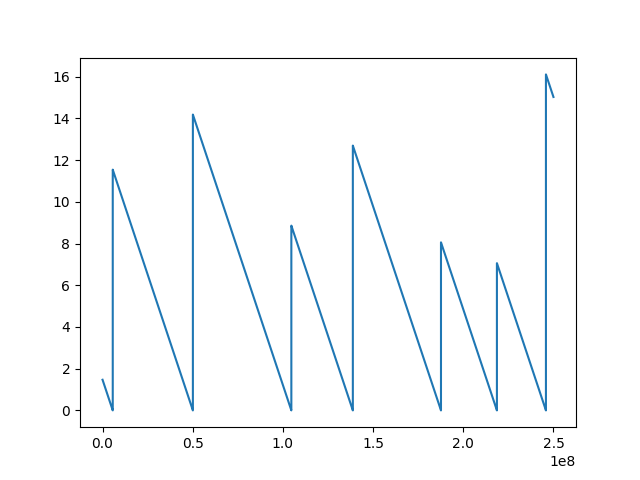
\includegraphics[width=\linewidth]{Figure_1.png}
  \caption{Graph of the time to failure of the seven earthquakes we are analyzing, x axis being time step and y axis being time to failure.}
  \label{fig:graph1}
\end{figure}

We realized that the LSTM generally learned all that it needed to before the first epoch was even halfway through, (as its accuracy didn't significantly improve from then on) so we used 2 epochs for training just in case.


\section{Results}

Our original LSTM had a correct prediction rate of 53 percent, while a arbitrary guessing would have given us about a 33 percent accuracy rate. We quickly strove to improve this score by changing the activation, loss, and optimizer functions (which we initially had as softmax, categorical\_crossentropy, and SGD). After some quick experimentation, we found that selu, cosine\_proximity, and Nadam seemed to work best for our network, raising our accuracy up to about 55\%.

In order to further attempt to improve our results, we then added the 7 manually added features to the LSTM. These features ended up only minimally improving the program by about 2 percent, ending the accuracy at about a 57 percent accuracy rate. 

Then, we added a 1D ConvNet layer to our LSTM to act as an initial feature detector. This step ended up giving a significant improvement of about 4 percent to the original LSTM, landing us at an accuracy of about 60 percent. 

Looking to increase our accuracy further, we looked at the discussion kernels on Kaggle. In regards to our manual features, we found a kernel in which an entrant had two-thousand features implemented into their LSTM. However, when we tried to increase the number of features on our feature detector to a number similar to this, we saw no improvement. Another kernel talked about the dangers of overfitting. Since the overall data only had 16 earthquakes, over analyzing the data may make the LSTM find patterns that are not there or are specific to those specific earthquakes that would impede on the overall results.

In some ours was an easier task than the original task (to predict TTF with a small degree of error) but it was also harder in that there
are very small margins between each discreet category. Incoming seismic waves four seconds away from an earthquake generally don't
seem to be that much different from waves three seconds to an earthquake, and as the predicted TTF nears the three or six second boundary
our model is punished more for small degrees of inaccuracy than a model tested on the original task. That said, the top kernels on Kaggle
are currently pushing 1.3\% mean-squared error on the given test data, so our model has a long way to go. 

 

\section{Conclusions}
We implemented an LSTM with a convolutional layer for feature detection to predict earthquake imminence based on small chunks of seismic data. We found that while hand-coded features, based on what we found important in the data, improved the LSTM's performance somewhat, a convolutional network that allowed it 
to determine its own features had by far the largest positive impact on performance. However, the top kernels on Kaggle for this problem all utilize massive sets of predetermined features from python statistics packages, so our results may have been the product of improper implementation. If we had more time, we would have liked to pursue the procedural generation direction mentioned briefly in the 
introduction, as that is one of the most interesting aspects to LSTMs and, we think, has the potential to be quite fruitful in respect
to these kinds of problems.


\end{document}

